\documentclass[presentation]{beamer}
\usetheme[
  subsectionpage=progressbar,
]{metropolis}           % Use metropolis theme

\usepackage{polyglossia}
\setdefaultlanguage{english}
\usepackage{fontspec}
\usepackage[final]{microtype}

\defaultfontfeatures{Ligatures=TeX}
\newfontfeature{Microtype}{protrusion=default;expansion=default}
\setmonofont{DejaVu Sans Mono}

\usepackage{listings}
\usepackage{graphicx}

\lstset{
  basicstyle=\footnotesize\ttfamily
}

\graphicspath{ {./images/} }

\title{Hacktoberfest}
\subtitle{Introduction to contributing to open source}
\date{13. oktober 2021}
\author{Sondre Nilsen, Anders Syvertsen}
\institute{echo makerspace}

\begin{document}
  \maketitle

  \begin{frame}
    \frametitle{Outline}
    \tableofcontents
  \end{frame}

  \section*{echo makerspace}
  \begin{frame}{echo makerspace}
    \begin{itemize}
      \item We run and organize the makerspace
      \item Organize events and teaching
      \item We need more people!
    \end{itemize}
  \end{frame}
  \begin{frame}[standout]
    \frametitle{echo makerspace}
    \LARGE{http://bit.ly/echomaker21}
  \end{frame}

  \section{Open Source}
  % Add communistic background image 
  \begin{frame}
    \frametitle{Open Source}
    \begin{itemize}
      \item React
      \item TypeScript
      \item Rust
      \item Linux
      \item Java/OpenJDK
      \item git
      \item Docker
      \item MySQL/PostgreSQL
      \item NodeJS
      \item ...many, many more
    \end{itemize}
  \end{frame}
  \begin{frame}
    \frametitle{Open Source}
 
    \begin{itemize}
      \item Software for the people, by the people
      \item Anyone can contribute and collaborate
      \item Modern IT wouldn't be possible without open source
      \item Many different licenses
      \begin{enumerate}
        \item MIT
        \item Apache
        \item GNU GPL
        \item EU PL
      \end{enumerate}
    \end{itemize}
  \end{frame}

  \begin{frame}
    \frametitle{Open Source}
 
    \centering
    
\includegraphics[width=0.7\textwidth]{hammer.png}
  \end{frame}

  \begin{frame}
    \frametitle{Open Source}
 
    \begin{itemize}
      \item Software for the people, by the people
      \item Anyone can contribute and collaborate
      \item Modern IT wouldn't be possible without open source
      \item Many different licenses
      \begin{enumerate}
        \item MIT
        \item Apache
        \item GNU GPL
        \item EU PL
      \end{enumerate}
    \end{itemize}
  \end{frame}

  \begin{frame}[standout]
    \frametitle{Choose a license}
    https://choosealicense.com/
  \end{frame}

  \section{Hacktoberfest}
  \begin{frame}[standout]
    \frametitle{Hacktoberfest}
  
    A way to pay back to the community \\

    https://hacktoberfest.com
  \end{frame}
  \begin{frame}
    \frametitle{Hacktoberfest}
  
    \begin{itemize}
      \item 4 PRs = swag/tree
      \item Must be contributing PRs, not wasteful
      \item Must be accepted
      \item Look for issues/repositories with \textbf{hacktoberfest} label
      \item Good way for budding developers to start contributing
    \end{itemize}
  \end{frame}

  \section{\texttt{git}}
  \begin{frame}
    \frametitle{\texttt{git}}
 
    \begin{itemize}
      \item Created by Linus Torvalds in a weekend for Linux development
      \item Most popular VCS for software development
      \item Used to keep track of changes for projects
      \item Enables decentralized contributing
      \item Useful for collaboration across teams and individuals
    \end{itemize}
  \end{frame}

  \subsection{Using \texttt{git}}
  \begin{frame}
    \frametitle{Workflow}
    
    \begin{enumerate}
      \item Project needs bug fixes, new features etc
      \item Checkout repository
      \item Create new branch
      \item Commit your changes as you work
      \item Push to remote repository
      \item Create pull request
      \item ??
      \item Profit
    \end{enumerate}
  \end{frame}
  \begin{frame}
    \frametitle{\texttt{git} commands}

    \begin{description}
      \item \texttt{git status}
      \item \texttt{git add ...}
      \item \texttt{git commit}
      \item \texttt{git commit -m "Message"}    
      \item \texttt{git push}
      \item \texttt{git pull}
      \item \texttt{git fetch}
      \item \texttt{git branch}
      \item \texttt{git switch}
      \item \texttt{git merge}
    \end{description}
  \end{frame}

  \begin{frame}[standout]
    \frametitle{git commands}
    https://git-man-page-generator.lokaltog.net/   
  \end{frame}

  \begin{frame}[fragile]
    \frametitle{\texttt{git status}}
 
    \begin{lstlisting}
$ git status
On branch main
Your branch is up to date with 'main'.

nothing to commit, working tree clean
    \end{lstlisting}
  \end{frame}

  \begin{frame}[fragile]
    \frametitle{\texttt{git branching}}
 
    \begin{lstlisting}
$ git branch
* main

$ git switch -c new-feature
Switched to a new branch 'new-feature'

$ git branch
  main
* new-feature
    \end{lstlisting}
  \end{frame}

  \begin{frame}[fragile]
    \frametitle{\texttt{git workflow}}
 
    \begin{lstlisting}
$ git status -s
 M presentation.tex

$ git add presentation.tex 

$ git status -s
M  presentation.tex

$ git commit -m "Add more frames about git workflow"
[new-feature c8b88d3] Add more frames about git workflow
 1 file changed, 76 insertions(+), 14 deletions(-)
    \end{lstlisting}
  \end{frame}

  \begin{frame}[fragile]
    \frametitle{\texttt{git pushing}}
 
    \begin{lstlisting}
$ git push -u origin new-feature
Enumerating objects: 5, done.
Counting objects: 100% (5/5), done.
Delta compression using up to 8 threads
Compressing objects: 100% (3/3), done.
Writing objects: 100% (3/3), 796 bytes | 796.00 KiB/s, done.
Total 3 (delta 2), reused 0 (delta 0), pack-reused 0
To github.com:echo-makerspace/hacktoberfest-2021.git
 * [new branch]      new-feature -> new-feature
Branch 'new-feature' set up to track remote branch 'new-feature' from 'origin'.

$ git status
On branch new-feature
Your branch is up to date with 'origin/new-feature'.
    \end{lstlisting}
  \end{frame}


  \subsection{Branching}
  \begin{frame}
    \frametitle{Branching}
  
    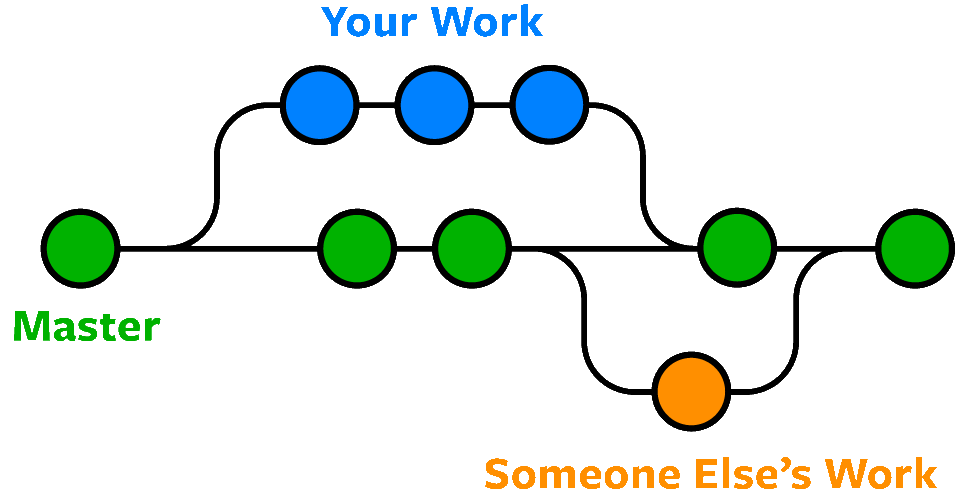
\includegraphics[width=\textwidth]{git-branches-merge.png}
  \end{frame}
  \begin{frame}
    \frametitle{Branching}
  
    \begin{itemize}
      \item Required for collaboration
      \item Useful for developing features in isolation
      \item Splitting production from development
    \end{itemize}  
  \end{frame}

  \subsection{Merging}
  \begin{frame}
    \frametitle{Merging}
  
    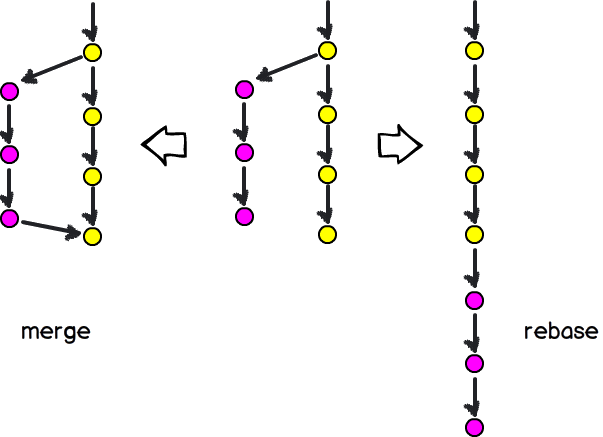
\includegraphics[width=\textwidth]{merge-vs-rebase.png}
  \end{frame}
  \begin{frame}
    \frametitle{Merging}
  
    \begin{itemize}
      \item Ask three developers, get four opinions
      \item Mostly a preference thing 
      \item Merging is not destructive
      \item Be careful with \texttt{rebase} if you're unfamiliar with it
    \end{itemize}
  \end{frame}

  \section{GitHub, GitLab, etc}
  \begin{frame}
    \frametitle{GitHub, GitLab}
  
    \begin{itemize}
      \item Platforms for collaborating using \texttt{git}
      \item Used by nearly everyone
      \item Tools for managing projects like issues, project boards, CI/CI etc
      \item Easy to use for collaboration
      \item Fork repositories to add own changes, create own project
      \item Send pull requests to add your changes
    \end{itemize}
  \end{frame}
  \begin{frame}
    \frametitle{Forking}
  
    
\includegraphics[width=\textwidth]{forking.png}
  \end{frame}
  \begin{frame}[standout]
    \frametitle{Protip}
 
    Use the GitHub CLI: \texttt{gh}
  \end{frame}

  \section{How to contribute?}
  \begin{frame}
    \frametitle{Contributing}
  
    \begin{itemize}
      \item Find repositories or issues with the \texttt{hacktoberfest} label
      \item Or \texttt{good-first-issue}
      \item Software you use but is missing a feature/has a bug
      \item Big or small, all good contributions are valuable
    \end{itemize}
  \end{frame}

  \section{DEMO}
  \section*{Pizza og jobbing}
\end{document}